% --------------------------------------------------------------
% This is all preamble stuff that you don't have to worry about.
% Head down to where it says "Start here"
% --------------------------------------------------------------
 
\documentclass[12pt]{article}
 
\usepackage{float} 
\usepackage[margin=1in]{geometry} 
\usepackage{amsmath,amsthm,amssymb}
\usepackage{listings}
\usepackage{enumitem}   
\usepackage{graphicx}
\graphicspath{ {./images/} }

\lstset{
   basicstyle=\fontsize{8}{9}\selectfont\ttfamily
}
 
\begin{document}
 
% --------------------------------------------------------------
%                         Start here
% --------------------------------------------------------------
 
%\renewcommand{\qedsymbol}{\filledbox}
 
\title{Homework 5}%replace X with the appropriate number
\author{Hai Nguyen \& Huan Nguyen\\ %replace with your name
STAT760 - Statistical Learning} %if necessary, replace with your course title
\maketitle
\textbf{Problem 1}

Initialization code:
\begin{lstlisting}
    clc
    clear all
    close all
    
    % Import data
    M = importdata("prostate.data");
    N_sample = length(M);
    
    % Exclude the first row (labels only)
    for i = 2 : N_sample - 1
        temp = cell2mat(M(i, :));
        temp = strsplit(temp);
        
        % Exclude index column (column 1), True/False column (last column)
        if i == 2
            data = str2double(temp(1, 2:end-1));  
        else
            data = [data; str2double(temp(1, 2:end-1))];
        end
    end
    
    % Total number of predictors
    p = 8;
\end{lstlisting}

\begin{enumerate}[label=\alph*)]
    \item Train a multivariate regression predictor for lpsa. Use the best subset selection method and plot the error rate for the best classifier (for 1, 2,...,8 predictors).
    
    Source code:
    
    \begin{lstlisting}
%% Best subset selection
% Fit all models
for k = 1:p
    total_models = combnk(1:p, k);
    
    [total_combination, width] = size(total_models);
    
    % Output
    y = data(:, end);
    
    max_Rsq = 0.0;
    best_feature = 9;
    
    for i = 1 : total_combination     
        % Construct vector X
        chosen_features = total_models(i, :);
        X = data(:, chosen_features);
        X = [ones(length(X),1) X];
        
        % Coefficient
        b = inv(X'*X) * X' * y;
        
        % Estimated output
        y_hat = X * b;
                
        % Calculate R^2
        Rsq = 1 - sum((y - y_hat).^2)/sum((y - mean(y)).^2);
        
        if Rsq > max_Rsq
            max_Rsq = Rsq;
            best_feature = chosen_features;
        end     
    end
    
    % Store best models with k predictors
    Model{k} = [max_Rsq best_feature];
end

% Select a single best model among saved models using adjusted R-squared
for index = 1:p
    % Retrieve R squared and the number of predictors used
    r_squared = Model{index}(1);
    n_predictor = length(Model{index}) - 1;
    
    % Calculate adjusted R squared
    adj_rsquared = 1 - (1-r_squared) * (N_sample - 1) / (N_sample - n_predictor - 1);
    
    % For plotting
    adj_R_squared(index) = adj_rsquared;
end

% Draw figure of adjusted R squared and the number of predictors
y_axis = 1:1:p;
plot(y_axis, adj_R_squared);
xlabel('Number of Predictors');
ylabel('Adjusted R^2');
grid on;
    \end{lstlisting}
    
   Plot of adjusted R squared and the number of predictors:
    
    \begin{figure}[H]
\begin{center}
  \caption{Adjusted R squared and the number of predictors}
  \label{Fig1}
  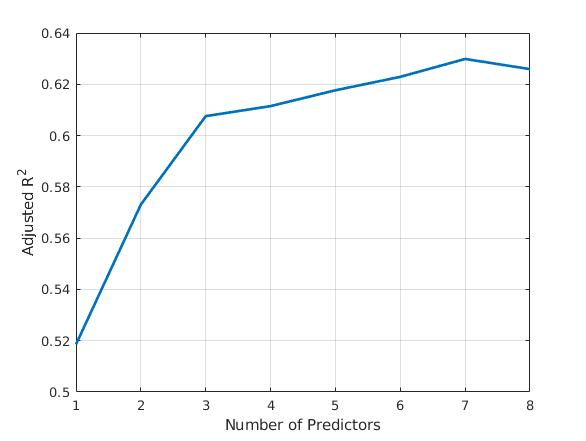
\includegraphics[width=0.5\textwidth]{images/Fig1.jpg}
 \end{center}
\end{figure}
    
    \item Train the same regression using ridge regression and plot the values of the coefficients
for different values of lambda (as in Fig. 6.4, left. Notice the log scale for lambda).

    Source code:
    
    \begin{lstlisting}
%% Ridge regression
% Normalize predictor
X_ridge = data(:, 1:end-1);
for col = 1:p
    mean_ = mean(X_ridge(:, col));
    std_  = std(X_ridge(:, col));
    X_ridge(:, col) = (X_ridge(:, col) - mean_)./std_;
end

y_ridge = data(:, end);
lambda = 0:1:10^4;

for index = 1:length(lambda)
    temp = inv(X_ridge' * X_ridge + lambda(index) * eye(p)) * X_ridge' * y_ridge;
    if index == 1
        b_ridge = temp;
    else
        b_ridge = [b_ridge temp];
    end
end

% Plot
semilogx(lambda, b_ridge, 'LineWidth', 2)
xlabel('Lambda')
ylabel('Standardized Coefficient')
legend('lcavol','lweight', 'age', 'lbph','svi','lcp','gleason', 'pgg45')
grid on
    \end{lstlisting}

Plot the values of the coefficients for different values of lambda.

    \begin{figure}[htb!]
\begin{center}
  \caption{Values of the coefficients for different values of lambda.}
  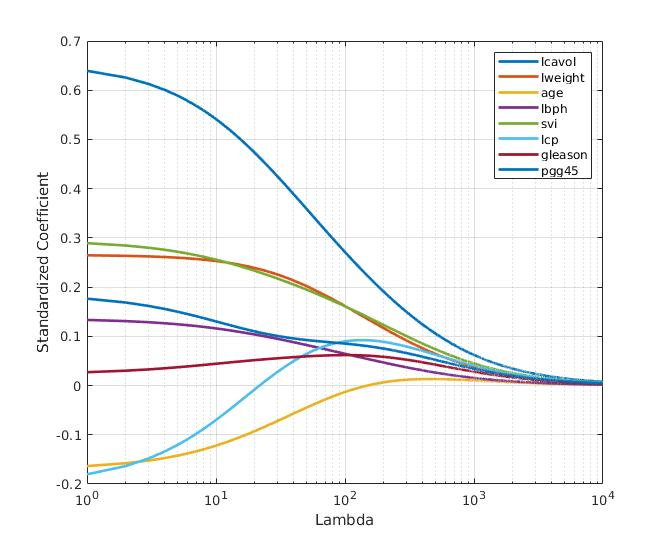
\includegraphics[width=0.75\textwidth]{images/Fig2.jpg}
 \end{center}
\end{figure}

    \item Train the same regression using the lasso (perform gradient descent and project the
vector of coefficients back into the feasible region at every step, if necessary). Use expression 6.8 and plot the value of the coefficients for different s.

Function gradient descent lasso:

\begin{lstlisting}
function [parameters,costHistory] = grad_descent_lasso(X, y, parameters, 
default_learningRate, num_iter, s)

m = length(y);

% Creating a matrix of zeros for storing our cost function history
costHistory = zeros(num_iter, 1); 

    for i = 1:num_iter        
    
        % Calculating the transpose of our hypothesis
        h = (X * parameters - y);        
    
        % Updating the parameters
        tmp_parameters = parameters - default_learningRate * (1/m) * X' * h;
        while (norm(tmp_parameters, 1) > s)
            default_learningRate = default_learningRate * 0.5;
            tmp_parameters = parameters - default_learningRate * (1/m) * X' * h;        
        end
        parameters = tmp_parameters;
        % Keeping track of the cost function
        costHistory(i) = 1/m*(X * parameters - y)'*(X * parameters - y);        
    end 
end
\end{lstlisting}

Use this function for lasso regression:

\begin{lstlisting}
X_lasso = [ones(size(data,1),1) X_ridge];
y_lasso = data(:, end);
s_array = [0.01 0.05 0.1 0.5 1 5 10];
b_lasso = [];
for i = 1:length(s_array)
    beta = zeros(size(X_lasso,2),1);
    [beta,costHistory] = grad_descent_lasso(X_lasso, y_lasso, beta, 0.1, 100, s_array(i));
    if index == 1
        b_lasso = beta;
    else
        b_lasso = [b_lasso beta];
    end   
end
figure
semilogx(s_array, b_lasso, 'LineWidth', 2)
xlabel('s')
ylabel('Standardized Coefficient')
legend('beta 0','lcavol','lweight', 'age', 'lbph','svi','lcp','gleason', 'pgg45')
grid on
\end{lstlisting}

Plot the value of coefficient for different s.

    \begin{figure}[H]
\begin{center}
  \caption{Values of the coefficients for different s.}
  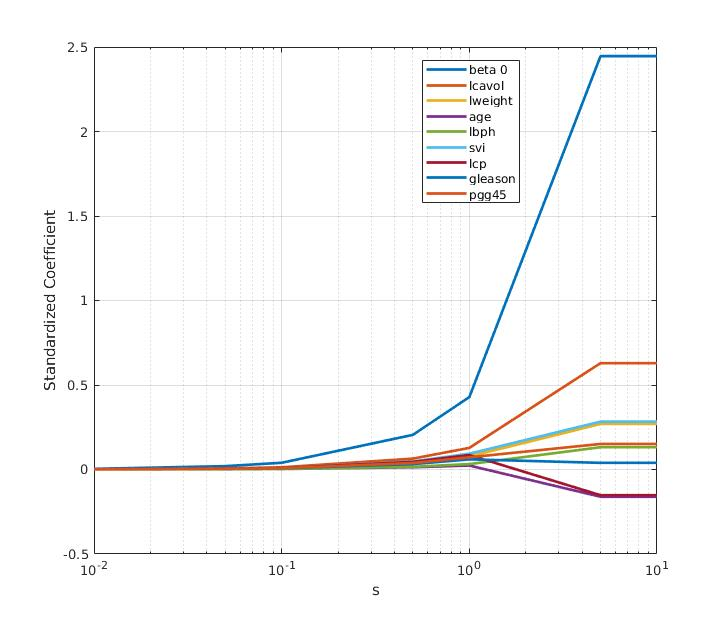
\includegraphics[width=0.75\textwidth]{images/Fig3.jpg}
 \end{center}
\end{figure}

\end{enumerate}
\textbf{Problem 2}
\begin{enumerate}[label=\alph*)]
   \item Correct answer is iii: The lasso, relative to least square, is less flexible and hence will give improved prediction accuracy when its increase in bias is less than its decrease in variance.\\
   The reason is because, lasso regression tries to limit the L1-norm of regression coefficient vector $\beta$, hence it is less flexible and will give higher bias than least square. But lasso will have smaller variance compare to least square. Since test error is the sum of bias, variance and irreducible error, if the increase in bias is less than the decrease in variance, lasso will give higher prediction accuracy. 
   \item Correct answer is iii: Ridge regression, relative to least square, is less flexible and hence will give improved prediction accuracy when its increase in bias is less than its decrease in variance.\\
   The reason is because, lasso regression tries to limit the L2-norm of regression coefficient vector $\beta$, hence it is less flexible and will give higher bias than least square. But lasso will have smaller variance compare to least square. Since test error is the sum of bias, variance and irreducible error, if the increase in bias is less than the decrease in variance, lasso will give higher prediction accuracy.
   \item
   Correct answer is ii: Non-linear methods, relative to least square, is more flexible and hence will give improved prediction accuracy when its increase in variance is less than its decrease in bias.\\
   The reason is because, least square uses linear model to predict the relationship between predictors and response, hence it is less flexible than non-linear methods which use non-linear model. As a result, non-linear methods will have smaller bias but higher variance compare to least square. Since test error is the sum of bias, variance and irreducible error, if the increase in variance is less than the decrease in bias, non-linear methods will give higher prediction accuracy than least square.   
\end{enumerate} 
\textbf{Problem 3}\\
   As s increase from 0
\begin{enumerate}[label=\alph*)]
   \item
   Training RSS will steadily decrease than remain constant. The reason is that when s increases, the feasible region expands and the model will be more flexible. When s is large enough, the optimal $\beta$ for training dataset will lie in feasible region and hence training RSS will achieve minimal value and remain constant as s increases. 
   \item
   Correct answer is ii: Test RSS decreases initially, and then eventually start increasing in a U shape. Test RSS is the sum of variance, squared bias and irreducible error. When s increases, the $L_1$-norm of regression coefficient vector $\beta$ is less restricted and the model is more flexible hence variance will increase and bias will decrease while irreducible error remains constant. When s is small, the increase in variance is lower than the decrease in bias, hence test RSS will decrease. When s is large enough, the increase in variance is higher than the decrease in bias, hence test RSS will increase.    
   \item 
   Correct answer is iii: Variance will steadily increase. The reason is that when s increases, the $L_1$-norm of regression coefficient vector $\beta$ is less restricted and the model is more flexible.
   \item 
   Correct answer is iv: Squared bias will steadily decrease. The reason is that when s increases, the $L_1$-norm of regression coefficient vector $\beta$ is less restricted and the model is more flexible.
   \item
   Correct answer is v: Irreducible error remains constant since it doesn't depend on the model.
\end{enumerate} 
% --------------------------------------------------------------
%     You don't have to mess with anything below this line.
% --------------------------------------------------------------
 
\end{document}